\documentclass[tikz,convert={outfile={test.svg}}]{standalone}
\usetikzlibrary{calc,intersections}

\begin{document}
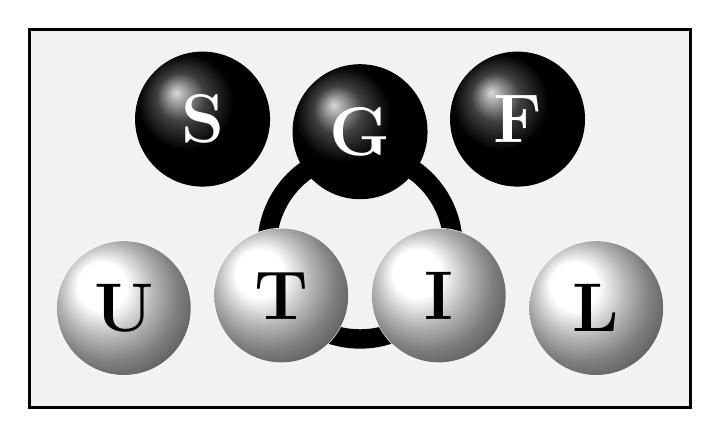
\begin{tikzpicture}
    \pgfmathsetmacro{\xhalf}{5}
    \pgfmathsetmacro{\xmargin}{0.8}
    \pgfmathsetmacro{\ylow}{1.5}
    \pgfmathsetmacro{\yhigh}{3.5}
    \pgfmathsetmacro{\tiltratio}{0.08}
    % Define points
    \coordinate (A) at ($(\xmargin,0)$);
    \coordinate (B) at ($(2*\xhalf-\xmargin,4.8)$);
    \foreach \x [count=\xi] in {U,S,T,G,I,F,L} {
        \pgfmathsetmacro{\xx}{\xi+1}
        \ifodd\xi
            \pgfmathsetmacro{\yy}{-abs(\xx-\xhalf)*\tiltratio+\ylow}
        \else
            \pgfmathsetmacro{\yy}{abs(\xx-\xhalf)*\tiltratio+\yhigh}
        \fi
        \coordinate (\x) at ($(\xx,\yy)$);
    }
    % Draw background
    \draw[very thick,fill=white!90!gray] (A) rectangle (B);
    % Draw a circle through points G, T, and I.
    \path[name path=Tc] (T) circle[radius=1];
    \path[name path=TI] (T) -- (I);
    \path[name path=TG] (T) -- (G);
    \path[name intersections={of=Tc and TI, by=cI}];
    \path[name intersections={of=Tc and TG, by=cG}];
    \coordinate (Tcm) at ($(cI)!0.5!(cG)$);
    \path[name path=Tr] (T) -- ($(Tcm)!-1.0!(T)$);
    \path[name path=H] (G) -- ($(T)!.5!(I)$);
    \path[name intersections={of=Tr and H, by=R}];
    \draw[line width=7pt] (R) let \p1 = ($(R) - (T)$)
        in circle[radius={veclen(\x1,\y1)}];

    % Draw 7 stones: 'SGFUTIL'.
    \foreach \x in {S,G,F} {
        \draw[fill=black] (\x) circle[radius=0.85];
        \shade[ball color=black] (\x) circle[radius=0.85] node[text=white] {\Huge\bfseries \x};
    }
    \foreach \x in {U,T,I,L} {
        \draw[draw=white, fill=white] (\x) circle[radius=0.85];
        \shade[ball color=white] (\x) circle[radius=0.85] node[text=black] {\Huge\bfseries \x};
    }
\end{tikzpicture}
\end{document}